\documentclass[onecolumn,10pt]{jhwhw}

\usepackage{epsfig} %% for loading postscript figures
\usepackage{amsmath}
\usepackage{graphicx}
\usepackage{grffile}
\usepackage{pdfpages}
\usepackage{algpseudocode}
\usepackage{wrapfig}
\usepackage{pgfplots}
\usepackage{amsfonts}
\usepackage{booktabs}
\usepackage{siunitx}
\usepackage{commath}
\usepackage{rotating}
\usepackage{url}
\usepackage{multimedia}
\usepackage{hyperref}

% Default fixed font does not support bold face
\DeclareFixedFont{\ttb}{T1}{txtt}{bx}{n}{12} % for bold
\DeclareFixedFont{\ttm}{T1}{txtt}{m}{n}{12}  % for normal

% Custom colors
\usepackage{color}
\usepackage{listings}
\usepackage{framed}
\usepackage{caption}
\usepackage{bm}
\captionsetup[lstlisting]{font={small,tt}}

\definecolor{mygreen}{rgb}{0,0.6,0}
\definecolor{mygray}{rgb}{0.5,0.5,0.5}
\definecolor{mymauve}{rgb}{0.58,0,0.82}

\lstset{ %
  backgroundcolor=\color{white},   % choose the background color; you must add \usepackage{color} or \usepackage{xcolor}
  basicstyle=\ttfamily\footnotesize, % the size of the fonts that are used for the code
  breakatwhitespace=false,         % sets if automatic breaks should only happen at whitespace
  breaklines=true,                 % sets automatic line breaking
  captionpos=b,                    % sets the caption-position to bottom
  commentstyle=\color{mygreen},    % comment style
  deletekeywords={...},            % if you want to delete keywords from the given language
  escapeinside={\%*}{*)},          % if you want to add LaTeX within your code
  extendedchars=true,              % lets you use non-ASCII characters; for 8-bits encodings only, does not work with UTF-8
  frame=single,                    % adds a frame around the code
  keepspaces=true,                 % keeps spaces in text, useful for keeping indentation of code (possibly needs columns=flexible)
  columns=flexible,
  keywordstyle=\color{blue},       % keyword style
  language=Python,                 % the language of the code
  morekeywords={*,...},            % if you want to add more keywords to the set
  numbers=left,                    % where to put the line-numbers; possible values are (none, left, right)
  numbersep=5pt,                   % how far the line-numbers are from the code
  numberstyle=\tiny\color{mygray}, % the style that is used for the line-numbers
  rulecolor=\color{black},         % if not set, the frame-color may be changed on line-breaks within not-black text (e.g. comments (green here))
  showspaces=false,                % show spaces everywhere adding particular underscores; it overrides 'showstringspaces'
  showstringspaces=false,          % underline spaces within strings only
  showtabs=false,                  % show tabs within strings adding particular underscores
  stepnumber=1,                    % the step between two line-numbers. If it's 1, each line will be numbered
  stringstyle=\color{mymauve},     % string literal style
  tabsize=4,                       % sets default tabsize to 2 spaces
}

\renewcommand{\lstlistingname}{Diagram}% Listing -> Algorithm

\author{John Karasinski}
\title{Homework 3}

\begin{document}
%\maketitle

\problem{Develop a very simple representation of the Hubble telescope.}
\begin{lstlisting}[caption={Hubble ASCII Diagram. Solar panel distance from HST is exaggerated. One character is $\approx$ 20 inches.}]
#########################################################################################
#                                         Hubble                                        #
#     ^V2                                                                               #
#     |                          +----------------------+                               #
#  <--+                          |                      |                               #
#  V1                            |         SA1          |                               #
#                                |                      |                               #
#                                +-----------+----------+                               #
#                                            |                                          #
#                                            |    +-------+                             #
#                             +--------------++---+       |                             #
#                             |               |   |       |                             #
#                             |       1       | 2 |   3   |                             #
#                             |               |   |       |                             #
#                             |               |   |       |                             #
#                             +--------------++---+       |                             #
#                                            |    +-------+                             #
#                                            |                                          #
#                                +-----------+----------+                               #
#                                |                      |                               #
#                                |         SA1          |                               #
#                                |                      |                               #
#                                +----------------------+                               #
#                                                                                       #
#########################################################################################
#                                                                                       #
#     ^V3                                                                               #
#     |                                                                                 #
#  <--+                                           +-------+                             #
#  V1                         +---------------+---+       |                             #
#                             |               |   |       |                             #
#                             |       1       | 2 |   3   |                             #
#                             |  +-----------+----------+ |                             #
#                             |               |   |       |                             #
#                             +---------------+---+       |                             #
#                                                 +-------+                             #
#                                                                                       #
#                                                                                       #
#                                                                                       #
#########################################################################################
\end{lstlisting}
% #                                                                                       #
% #     ^V3                                                                               #
% #     |                                                                                 #
% #  <--+                         +---+                  +---+                            #
% #  V2                           |   |                  |   |                            #
% #                               |   |     ________     |   |                            #
% #                               |   |    /  *--*  \    |   |                            #
% #                               |   |   / *      * \   |   |                            #
% #                               |   +--| *        * |--+   |                            #
% #                               |   |   \ *      * /   |   |                            #
% #                               |   |    \  *--*  /    |   |                            #
% #                               |   |      ------      |   |                            #
% #                               |   |                  |   |                            #
% #                               +---+                  +---+                            #
% #                                                                                       #
% #                                                                                       #
% #########################################################################################

\begin{figure}[h!]
\begin{center}
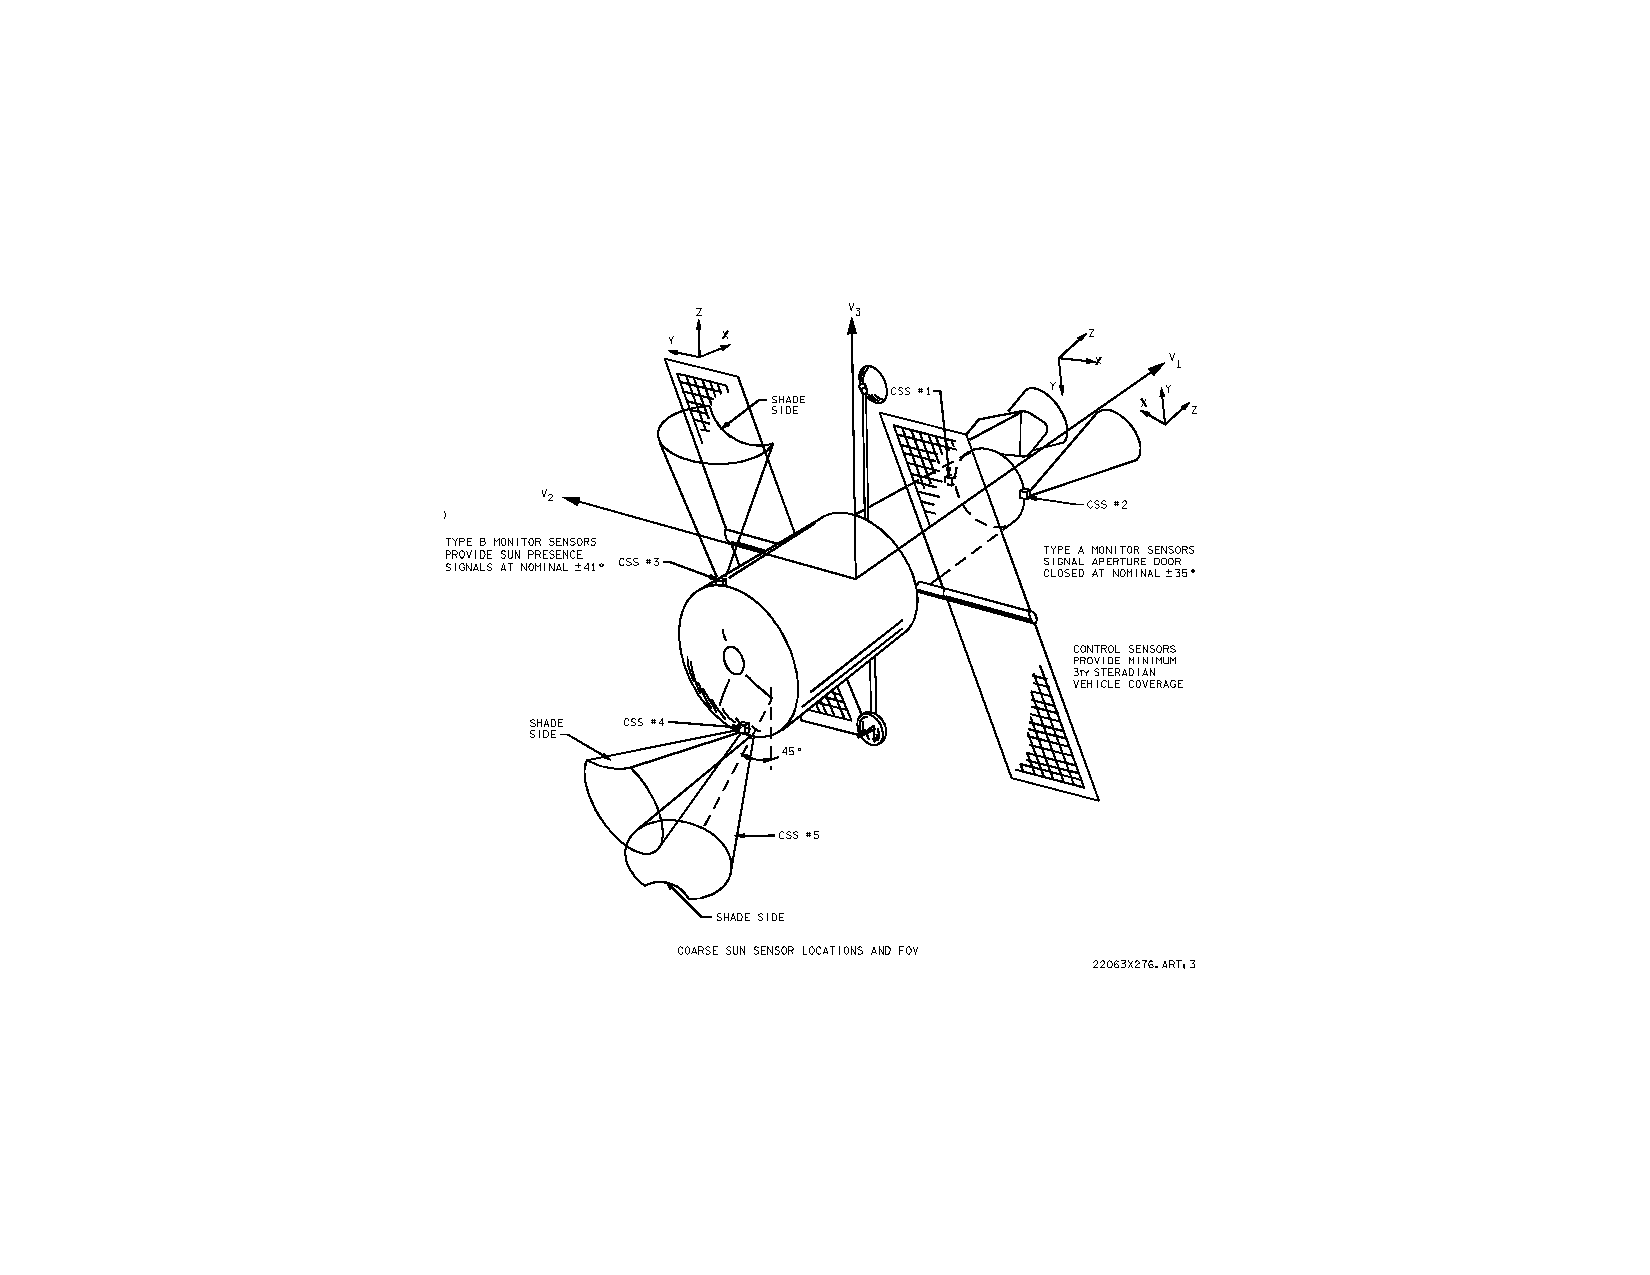
\includegraphics[height=0.45\textheight]{hst_axes.pdf}
\label{fig:on}
\end{center}
\caption{HST Axes Definition for $V_1, V_2, V_3$, CG is located at axis origin}
\end{figure}

We model both the body (3 sections) and the solar panels (2 sections) of the Hubble Space Telescope (HST). The body sections are connected as such: Section 1 is connected to Section 2, and Section 2 is connected to Section 3. The solar arrays are connected on Section 1, along the centerline, 20.75 inches $V_1$ away from the connection point with Section 2, and the near edge of the SA is 129 inches from center of Section 1. These sections are modelled with thin walled cylinders (TWC), solid cylinders (SC), and flat plates (FP). The rough layout of the sections is shown on the previous page, and the mass and length properties of each section are listed in Table~\ref{properties}.

\begin{table}[h!]
\begin{center}
\begin{tabular}{l r r r r r}
\toprule
Section & Model & $V_1$ (in) & $V_2$ (in) & Weight (lb) \\
\midrule
\it{Section 1} & & & & \\
\hspace{1em} Light Shield (LS)   & - & 153.2  & 120  & - \\
\hspace{1em} Forward Shell (FS)  & - & 156.05 & 121.2 & - \\
\hspace{1em} Total  & TWC & 309.25 & 121.2 & 9033 \\
\it{Section 2} & & & & \\
\hspace{1em} SSM Equipment Section (SSM-ES) & TWC &  61.25  &  121.2 & 10593\\
\it{Section 3} & & & & \\
\hspace{1em} Aft Shroud (AS) & SC &  138.00  &  168.16 & 3363\\
\it{Section 4} & & & & \\
\hspace{1em} Solar Arrays (SA) & FP &  476.8$^1$  &  113.5 & 735$^2$\\
\bottomrule
\end{tabular}
\end{center}
\caption{$^1$: This length can be fully rotated into $V_3$. $^2$: Weight of both solar arrays. $V_1$ and $V_2$ indicate the measurements of the parts. All lengths taken from Hubble technical drawings,  NASA, ``Cargo Systems Manual (CSM): Hubble Space Telescope,'' February 13, 2002; all masses from Mattice, J., ``Hubble Space Telescope Systems Engineering Case Study.''}
\label{properties}
\end{table}

\clearpage
\problem{Use this model as a basis to write a function(s) to determine the Mass Center and Inertia Matrix for any location.}

Using the radial-center of the farthest tip of Section 1 as our zero point , the center of mass is located at $V = [282, 0, 0]$ inches. This makes since, as the model is symmetric about the $V_2$ and $V_3$ axes, and the center of mass of the solar arrays is calculated to be $\approx 288$ inches along $V_1$.

The HST inertia matrix\footnote{Queen, S., ``HRV GNC Peer Review, Flight Performance Analysis,'' Tech. rep., NASA Goddard Space Flight Center, 2004.}, was at one point measured as:
\begin{align*}
I =
\begin{bmatrix}
    36046       & -706  &  1491 \\
    -706        & 86868 &   449 \\
    1491        & 449   & 93848
\end{bmatrix}
kg \cdot m^2.
\end{align*}
The Python script in Appendix gives the result of:
\begin{align*}
I =
\begin{bmatrix}
   43535 &      0 &      0 \\
       0 & 117651 &      0 \\
       0 &      0 & 135519
\end{bmatrix}
kg \cdot m^2,
\end{align*}
which has a relative error of:
\begin{align*}
I =
\begin{bmatrix}
  -20, 100, 100 \\
100,   -35, 100 \\
100, 100, -44
\end{bmatrix}
\%.
\end{align*}
Note that while our simple, 5 part model does a very good job of predicting the $I_{V_1}$ component ($\approx20$\% error), the $I_{V_2}$ and $I_{V_3}$ components are not represented very well. This is likely due to leaving out the antenna booms, which should have the largest effect in the $V_2$ and $V_3$ directions. It should also be noted that, due to the symmetric nature of our model, all of the off-axis terms are missing.

\begin{figure}[h!]
\begin{center}
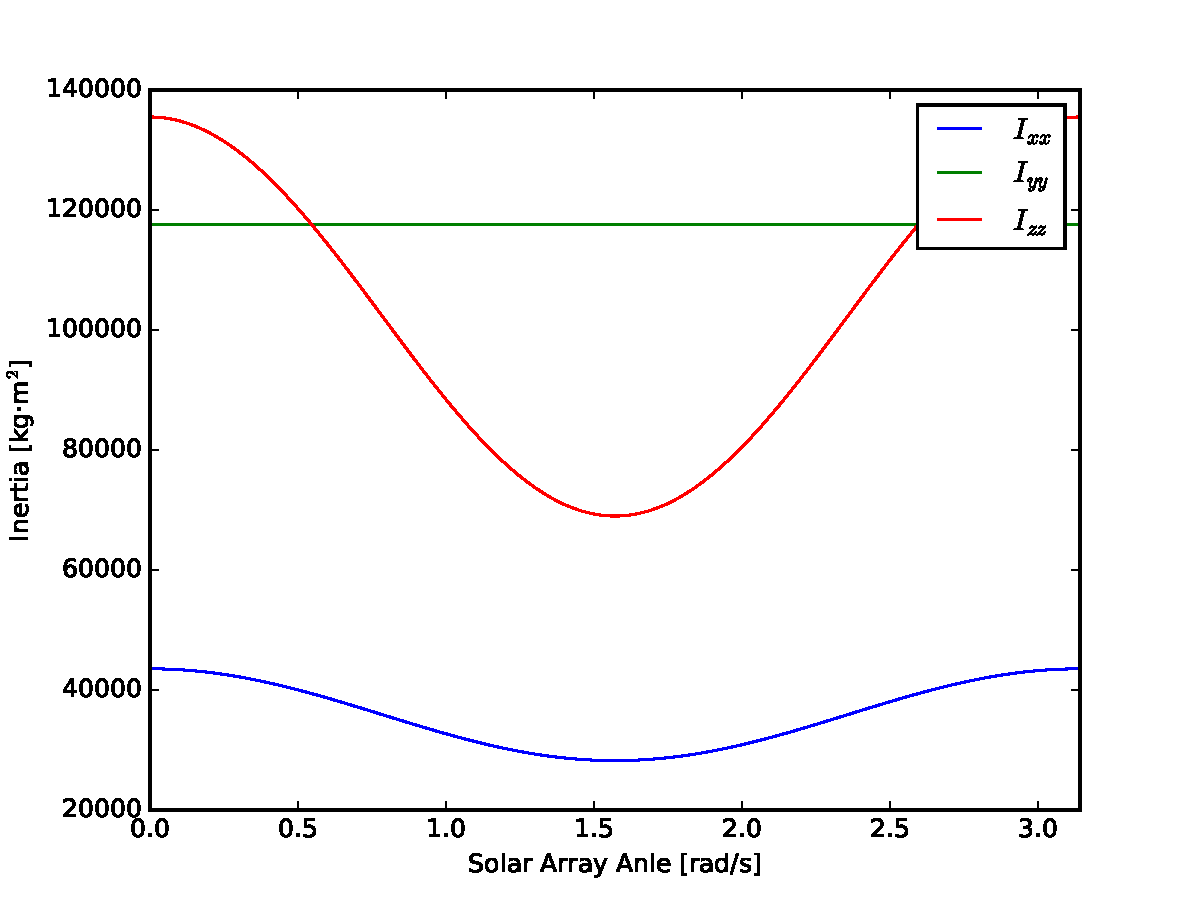
\includegraphics[height=0.45\textheight]{figure1.pdf}
\label{fig:on}
\end{center}
\caption{Inertias for principal axes for different solar array configurations}
\end{figure}

\clearpage
\problem{Write a function to find the current angular momentum relative to the mass center.}
\begin{figure}[h!]
\begin{center}
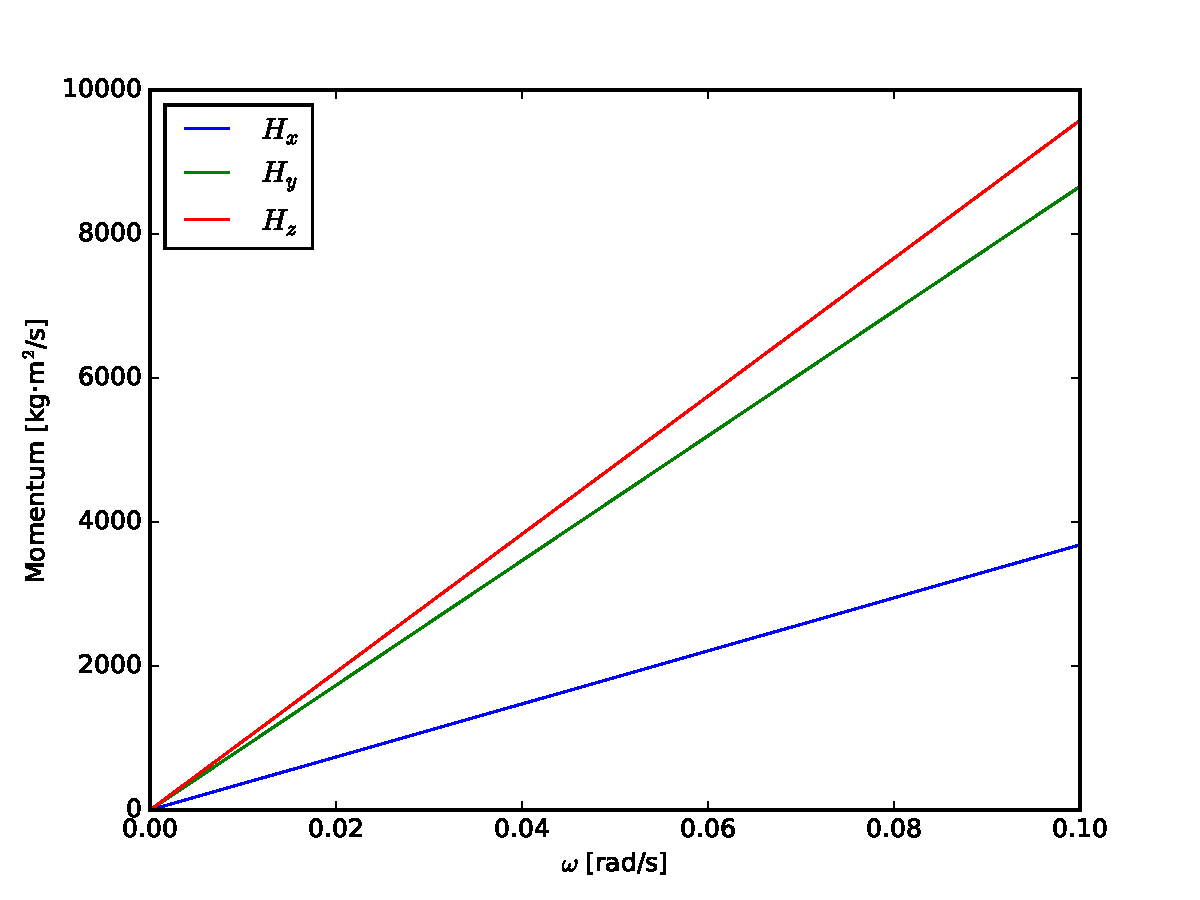
\includegraphics[height=0.45\textheight]{figure2.pdf}
\label{fig:on}
\end{center}
\caption{Effects of spin on each axis}
\end{figure}

\clearpage
\problem{Choose the optimal location for a torque producing system and explain why you think is the best location.}

\clearpage
\problem{Using your previous functions, write a program to find the resulting angular acceleration produced from a given torque.}

\clearpage
\problem{Write what next steps you would take to develop a controller that keeps the craft pointed in a specific direction.}

\end{document}
